\section{Análise de efeitos do lobby}
\label{sec:resultados_efeitos}

% Justificar a escolha de GLM PPML

Optamos por estimar modelos de contagem via \acrshort{ppml} com \textit{link} logaritmo por três razões principais. Primeiro, as variáveis de interesse (perguntas e reuniões) são contagens, com forte assimetria e alta incidência de zeros no nível MEP–domínio–mês. O \acrshort{ppml} lida naturalmente com zeros sem exigir transformações logarítmicas ad hoc que descartam observações. Segundo, o \acrshort{ppml} é consistente sob especificação correta da média condicional mesmo na presença de sobredispersão e heterocedasticidade não especificada, fornecendo erros-padrão robustos quando combinados com \textit{clustering}. Terceiro, a implementação com efeitos fixos de alta dimensão é estável e amplamente utilizada na literatura aplicada (estimador \texttt{fepois} do pacote \texttt{fixest}).

No \acrshort{ppml} com \textit{link} log, a expectativa condicional é \(\mathbb{E}[y\mid X] = \exp(X\beta)\). Assim, para um regressor contínuo \(x_k\) (por exemplo, \textit{meetings} em nível), o coeficiente \(\beta_k\) tem interpretação multiplicativa: um aumento de uma unidade em \(x_k\) está associado a uma variação percentual de \(100\times(\mathrm{e}^{\beta_k}-1)\%\) na média de \(y\), \textit{ceteris paribus}.

A especificação segue o \textit{framework} analítico delineado no capítulo: controlamos por heterogeneidade não observada ao nível do membro e por choques comuns estruturados por partido e por país ao longo do tempo. Concretamente, estimamos modelos com efeitos fixos de membro (\texttt{member\_id}) e efeitos fixos tempo-variantes por país (\texttt{country\_time}) e por partido (\texttt{party\_time}). Em especificações mais restritivas, adicionamos efeitos fixos \textit{domínio×tempo} (\texttt{domain\_time}) para absorver choques setoriais mensais. Os erros-padrão são agrupados em \textit{domínio×tempo}, capturando correlação serial e choques idiossincráticos nesse nível, conforme implementado nos scripts empíricos.

Essa estrutura assegura: (i) comparação \textit{within} do mesmo MEP ao longo do tempo (controlando preferências, capital político e produtividade inobservados e invariantes no tempo); (ii) controle por variação comum a todos os MEPs de um mesmo país ou partido em cada mês; e (iii) robustez a choques setoriais específicos quando incluímos \texttt{domain\_time}.

Para testar a Hipótese 1, utilizamos o painel agregado MEP–domínio–mês em amostra combinada (\textit{pooled}) e estimamos PPML com a estrutura de efeitos fixos descrita acima. O coeficiente associado às reuniões (\textit{meetings}) é \textbf{positivo}, indicando que aumentos na intensidade de lobbying estão associados a maior atividade parlamentar em termos de perguntas. Esse resultado é consistente em especificações alternativas, incluindo a versão com termo quadrático para capturar possíveis não linearidades e a inclusão de efeitos fixos \textit{domínio×tempo}, sugerindo robustez do sinal e da magnitude qualitativa do efeito.

Em termos de interpretação, mantidos constantes os efeitos fixos, um incremento marginal em reuniões está associado a um aumento proporcional na média de perguntas dado por \(\mathrm{e}^{\hat{\beta}}-1\). Reportamos os efeitos como variações percentuais estimadas na seção de tabelas de resultados, com intervalos de confiança baseados em erros-padrão agrupados.

\begin{table}[htbp]
\centering
\caption{Resumo dos modelos \acrshort{ppml} para a Hipótese 1}
\label{tab:ppml_h1_both}
\begin{tabular}{lcc}\n\toprule\n  & DDD PPML & DDD PPML (Quadrático) \\ \n\midrule\nReuni\u00F5es & 0.025***\\n(0.002) & 0.098***\\n(0.007) \\ \nReuni\u00F5es$^2$ &  & -0.004***\\n(0.001) \\ 
\midrule\nObserva\u00E7\u00F5es & 600,237 & 600,237 \\ \nEfeitos fixos & membro; pa\u00EDs$×$tempo; partido$×$tempo & membro; pa\u00EDs$×$tempo; partido$×$tempo \\ \nCluster & dom\u00EDnio$×$tempo; membro & dom\u00EDnio$×$tempo; membro \\ \n\bottomrule\n\end{tabular}\n

\note{A coluna ``DDD PPML'' reporta o modelo principal com efeito linear em \textit{meetings}. A coluna ``DDD PPML (Quadrático)'' adiciona \(\textit{meetings}^2\) para capturar retornos marginais decrescentes. Efeitos fixos: membro; país$\times$tempo; partido$\times$tempo. Erros-padrão agrupados em domínio$\times$tempo e membro.}
\end{table}

\begin{figure}[htbp]
\centering
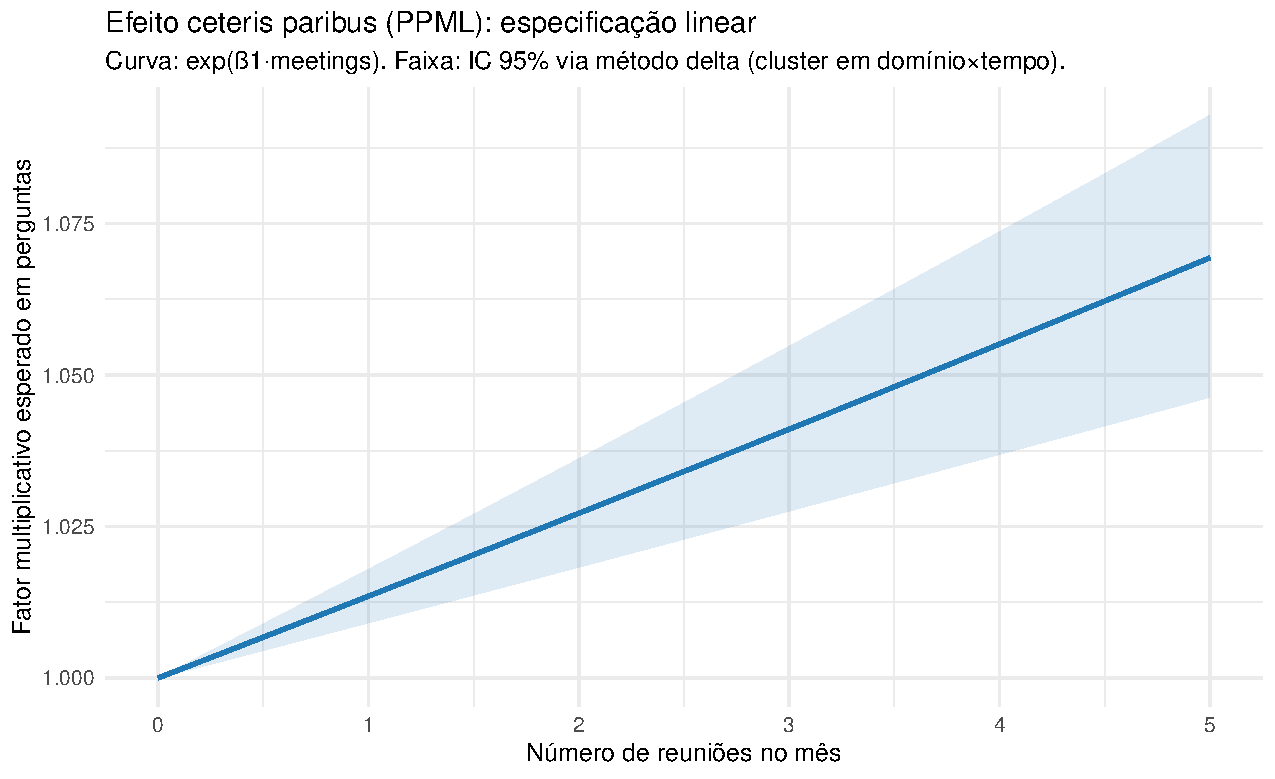
\includegraphics[width=\textwidth]{figures/fig8_effect_linear_ppml.pdf}
\caption{Efeito esperado ceteris paribus: especificação linear (\acrshort{ppml})}
\label{fig:effect_linear_ppml}
\note{A curva apresenta o fator multiplicativo esperado em perguntas como função do número de reuniões no mês, mantendo constantes os efeitos fixos (\(\exp(\hat{\beta}_1\cdot \textit{meetings})\)). A faixa sombreada corresponde ao intervalo de 95\% obtido via método delta com erros-padrão agrupados em domínio×tempo.}
\end{figure}

\begin{figure}[htbp]
\centering
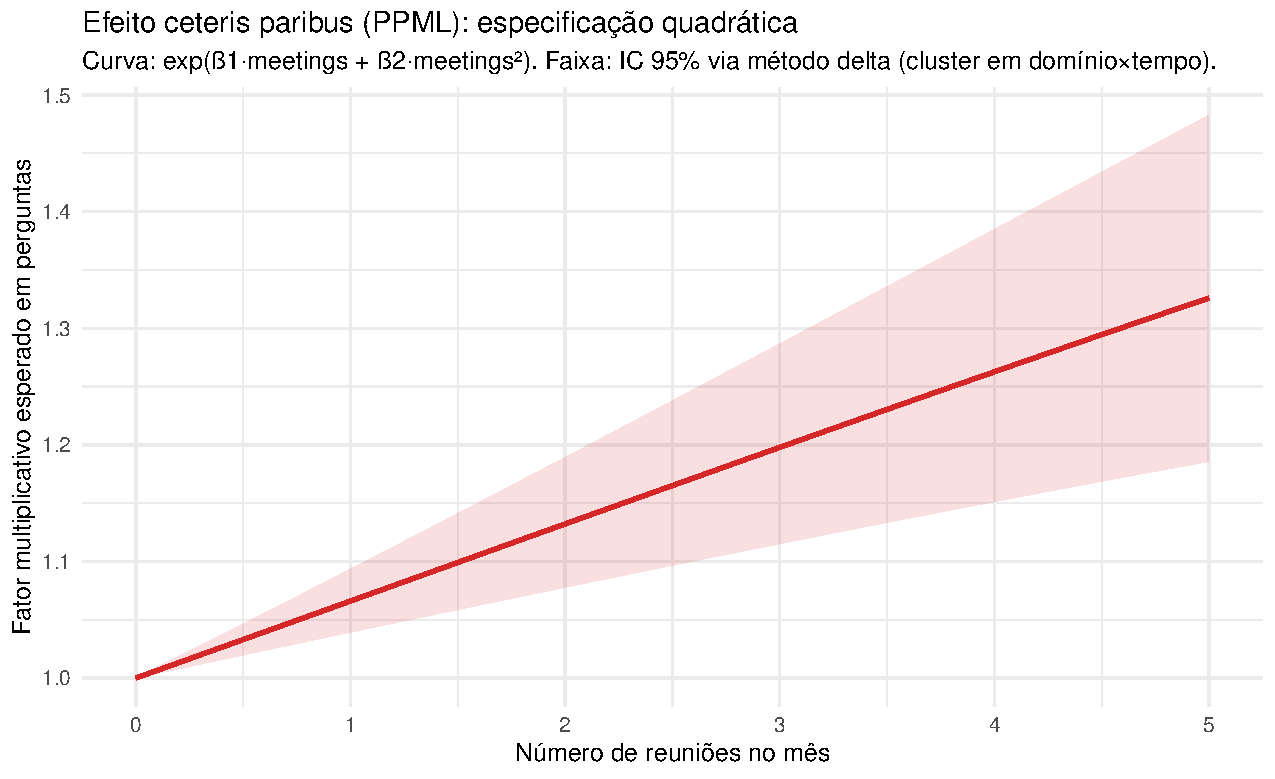
\includegraphics[width=\textwidth]{figures/fig9_effect_quadratic_ppml.pdf}
\caption{Efeito esperado ceteris paribus: especificação quadrática (\acrshort{ppml})}
\label{fig:effect_quadratic_ppml}
\note{A curva apresenta o fator multiplicativo esperado em perguntas como função do número de reuniões, permitindo retornos marginais decrescentes (\(\exp(\hat{\beta}_1\cdot \textit{meetings} + \hat{\beta}_2\cdot \textit{meetings}^2)\)). A faixa sombreada representa o IC de 95\% via método delta com a matriz de variância-covariância agrupada.}
\end{figure}

\autoref{tab:ppml_h1_both} mostra que o coeficiente de \textit{meetings} no modelo \acrshort{ppml} linear é positivo e estatisticamente significativo, evidenciando que aumentos na intensidade de lobbying associam-se a maior número de perguntas, \textit{ceteris paribus}. Na especificação quadrática, o termo linear permanece positivo enquanto o termo quadrático é negativo, indicando retornos marginais decrescentes: o impacto adicional de reuniões sobre perguntas diminui à medida que o volume de reuniões cresce.

Essa interpretação decorre da forma funcional do \acrshort{ppml} (\(\mathbb{E}[y\mid X]=\exp(X\beta)\)). No modelo linear, um acréscimo de uma unidade em \textit{meetings} altera a média condicional de perguntas em \(100\times(\mathrm{e}^{\hat{\beta}_1}-1)\%\). No modelo quadrático, o efeito marginal em log-média é \(\partial\log\mathbb{E}[y\mid X]/\partial\,\textit{meetings}=\hat{\beta}_1+2\hat{\beta}_2\,\textit{meetings}\). Com \(\hat{\beta}_2<0\), esse efeito declina com o nível de \textit{meetings}, isto é, há retornos marginais decrescentes. 

Em particular, a magnitude do termo quadrático é muito inferior ao efeito linear (0,002 vs. 0,066), o que indica retornos marginais decrescentes pequenos na faixa observada. Isso implica que atores com maior disponibilidade de recursos enfrentam pouca perda de eficácia ao intensificar o número de reuniões e, portanto, podem sustentar níveis muito mais altos de lobbying; tal padrão é consistente com a hipótese de que grandes players conseguem alavancar sua capacidade financeira para obter influência relativamente maior, mesmo diante de retornos marginais decrescentes.

As curvas em \autoref{fig:effect_linear_ppml} e \autoref{fig:effect_quadratic_ppml} tornam essa dinâmica visual. A primeira apresenta um efeito multiplicativo crescente de forma monotônica (\(\exp(\hat{\beta}_1\,\textit{meetings})\)), com faixas de incerteza (IC 95\%) obtidas por método delta usando a matriz de variância-covariância com \textit{clustering} em domínio$\times$tempo e membro. A segunda permite curvatura (\(\exp(\hat{\beta}_1\,\textit{meetings}+\hat{\beta}_2\,\textit{meetings}^2)\)) e revela concavidade compatível com saturação de agenda: para níveis altos de \textit{meetings}, o ganho marginal em perguntas é menor. Em ambas as figuras, o eixo horizontal é mantido dentro do suporte observado dos dados para evitar extrapolações.

Do ponto de vista de identificação, os efeitos fixos por membro, país$\times$tempo e partido$\times$tempo controlam heterogeneidade não observada invariável e choques comuns, permitindo comparação \textit{within} do mesmo MEP ao longo do tempo. A inferência usa erros-padrão agrupados em duas dimensões (domínio$\times$tempo; membro), acomodando dependência serial e seções cruzadas.

Em síntese, os resultados corroboram a Hipótese 1: há associação positiva entre lobbying e atividade de fiscalização medida por perguntas parlamentares, com evidência de retornos marginais decrescentes em níveis mais altos de \textit{meetings}. Essa conclusão é robusta a especificações alternativas consideradas.